\documentclass[conference]{IEEEtran}
\IEEEoverridecommandlockouts
% The preceding line is only needed to identify funding in the first footnote. If that is unneeded, please comment it out.
\usepackage{cite}
\usepackage{amsmath,amssymb,amsfonts}
\usepackage{algorithmic}
\usepackage{graphicx}
\usepackage{textcomp}
\usepackage{xcolor}
\usepackage[spanish]{babel}

\def\BibTeX{{\rm B\kern-.05em{\sc i\kern-.025em b}\kern-.08em
    T\kern-.1667em\lower.7ex\hbox{E}\kern-.125emX}}
\begin{document}

\title{Trabajo Práctico "Disipadores"\\
{\footnotesize \textsuperscript{}Curso 2023 - Tecnología de los Materiales Electrónicos}
\thanks{}
}

\author{\IEEEauthorblockN{1\textsuperscript{st} Ramiro Belsito}
\IEEEauthorblockA{\textit{Estudiante} \\
\textit{Instituto Tecnológico de Buenos Aires}\\
Buenos Aires, Argentina\\
rabelsito@itba.edu.ar}
\and
\IEEEauthorblockN{2\textsuperscript{nd} Facundo Caviglia}
\IEEEauthorblockA{\textit{Estudiante} \\
\textit{Instituto Tecnológico de Buenos Aires}\\
Buenos Aires, Argentina \\
fcaviglia@itba.edu.ar}}

\maketitle


\begin{abstract}
En el siguiente informe se analizará la utilidad de dos disipadores proveídos por la cátedra
para el buen funcionamiento de un regulador de tensión con encapsulado TO220.
\end{abstract}

\section{Introduction}
Se analizará la resistencia térmica de estos por medio de la práctica y se comparará con los valores 
obtenidos por medio de las ecuaciones teóricas y la hoja de datos del fabricante. Con estos datos
se realizará el circuito térmico equivalente y se intentará realizar simulaciones para poder contrastar
los resultados obtenidos empíricamente. Además se estudiará la influencia del posicionamiento del disipador,
frente a la posición óptima.

\section{Forma y Dimensiones}
\begin{figure}[h]
    \centering
    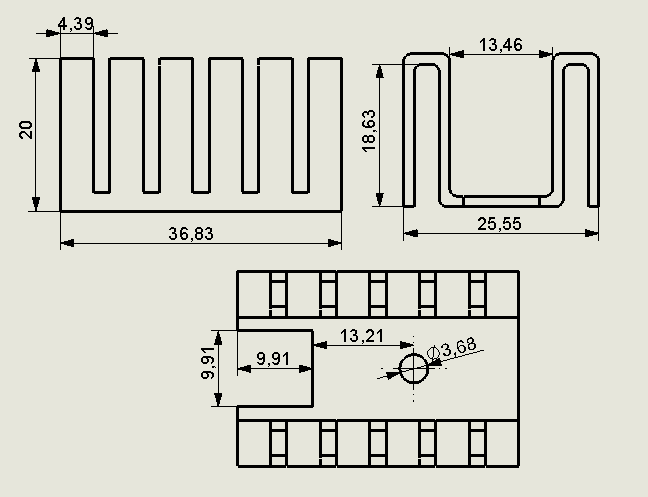
\includegraphics[width=0.3\textwidth]{PlanoRamiCompleto.png}
    \caption{Plano del disipador 1}
    \centering
    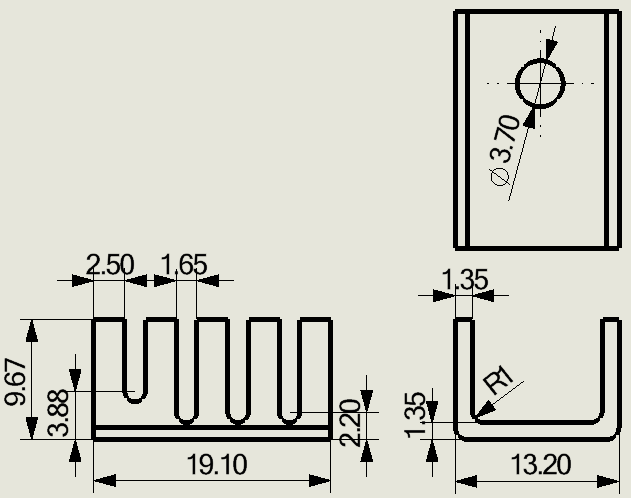
\includegraphics[width=0.3\textwidth]{disipadorFacu.png}
    \caption{Plano del disipador 2}
\end{figure}
Ambos disipadores son estampados sobre una plancha de aluminio anodizado, y luego tratado con otros 
procesos mecánicos para obtener la forma de cada uno. Por su método de fabricación cada disipador
es una pieza única, a diferencia de los fabricados por extrusión, que son piezas continuas cortadas 
a la medida requerida

\section{Cálculos Teóricos}
\subsection{Disipador 1}

La superficie de contacto, obtenida a través del modelado en Solidworks, es de 6915,40$m^2$.

\section{Mediciones Experimentales}
A continuacion


\end{document}
